\section*{What Is a Star Tracker and How Do They Work?}
\par \qquad A star tracker is an optical-based sensor that uses the position of stars to determine its attitude; it relies on the notion that relative star movement is low and can be effectively mapped to each other.
This mapping exists within catalogs formulated over several years from different organizations such as the Yale Bright Star Catalog 5 (BSC5). 
The catalog contains key information such as Star ID, right ascension and declination in the celestial sphere, brightness magnitude, right ascension and declination motion, and other features.

\begin{figure}[h]
    \begin{adjustbox}{center}
\begin{tabular}{|| c c c c c c c c c ||}
    \hline
    \thead{Catalog\\Number} & \thead{B1950 Right\\Ascension} & \thead{B1950\\Declination} & \thead{Spectral\\Type} & \thead{V Magn.\\ x100} & \thead{R.A. Proper\\Motion} & \thead{Dec.Proper\\Motion} & \thead{Radial\\Velocity} & \thead{Object\\Name} \\ [0.5ex] 
    \hline\hline

    & & & & \dots & & & & \\ 
    \hline
    123 & 0.138637 & 0.951592 & B8 & 4.73 & 2.181662e-07 & -4.848137e-08 & - & - \\
    \hline
    124 & 0.138259 & 0.922222 & K2 & 5.60 & -2.569512e-07 & -9.211460e-08 & - & - \\
    \hline
    125 & 0.137081 & -0.851784 & A0 & 4.77 & 6.932835e-07 & 8.241832e-08 & - & - \\
    \hline
    & & & & \dots & & & & \\ 
    \hline

\end{tabular}
\end{adjustbox}
\caption{Sample star catalog entry from Yale Bright Star Catalog}
\end{figure}

\par \qquad A copy of the catalog can then be modified to include information, called features, such as inter-star angles, ratio of triangle legs created by 3 stars, or even pyramidal information; the specific feature generated is determined by the specific identification method employed.
The modified catalog contains the permutations of the stars that comprise the given feature set.
The identification algorithm can then be used to identify each star in a given image; once each star is identified, a final calculation to determine the star location and the center of the image is processed and mapped to the original catalog.
Given the position of the star in the image, the star tracker can determine its own position (in right ascension and declination) based on the image center (as this is where the boresight of the star tracker lies).
The QUEST algorithm can then be used to determine a quaternion representation of the star tracker's attitude from the right ascension and declination.

\begin{figure}[h]
    \begin{adjustbox}{center}
\begin{tabular}{|| c c c ||}
    \hline
    Star A ID & Star B ID & $cos($Inter-star Angle$)$ \\
    \hline\hline

    & \dots & \\ 
    \hline
    123 & 124 & - \\
    \hline
    123 & 125 & - \\
    \hline
    124 & 125 & - \\
    \hline
    & \dots & \\ 
    \hline

\end{tabular}
\end{adjustbox}
\caption{Sample modified star catalog using inter-star angle identification}
\end{figure}

\par \qquad Onboard the star tracker, images are captured of the stars and processed by the star tracker.
During the centroiding process, the star tracker will read the image and determine where the stars are located within the image plane.
It will then create the aforementioned features and store it in memory.
During the identification process, the features in memory are recalled and compared to against the modified catalog where potential matches are found.
Once a suitable match, typically characterized by high likelihood of similarity in combination with a filter, the attitude is recalled from the entry in the modified catalog.
It is not uncommon for the star tracker to fail in finding a sufficiently confident match due to the nigh-infinite number of variations a single feature set can have due to image positioning and centroiding errors.
To combat this, star trackers typically take multiple images per second to try to find better matches.
This process repeats indefinitely and will generate high-accuracy determinations of attitude.

\begin{figure}[h]
    \begin{adjustbox}{center}
        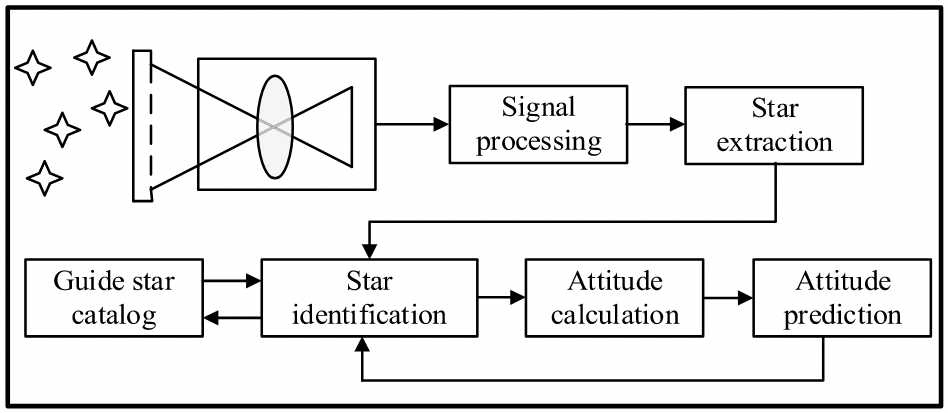
\includegraphics[scale=0.45]{star_tracker_process.png}
    \end{adjustbox}
    \caption{Working principle of the star tracker system \cite{rolling_shutter_errors}}
\end{figure}

\par \qquad The star tracker, in addition to its 2 main process phases, has 2 operating phases.
If the star tracker has some \emph{a priori} knowledge of its attitude in recent time, i.e., based on previous star tracker readings, then the star tracker only has to search a small portion of the modified catalog in order to find a match as the catalog can be ordered by attitude.
If, however, the star tracker has no \emph{a priori} knowledge of its attitude, i.e., post-detumble, then the star tracker must search the entire modified catalog.
Because the modified catalog is so large and can contain a great number of combinations for an even greater number of stars, the process to determine the attitude can take significantly longer.
This operating phase is typically called the \emph{Lost in Space} problem and is a unique metric in comparing star tracker performance.

\par \qquad \emph{Flowchart of entire star tracker process including Lost in Space problem}
